\section{Ghost}
\label{sec:CMS_ghost}

Ghost is a fully featured blogging platform built entirely with JavaScript.
Ghost is a Node.js application powered by the Express framework. Ghost ships with SQLite, and everything is connected through JugglingDB ORM.

Ghost is available via NPM, so it’s really easy to install on major environments.
Ghost theming is done with Handlebars, which keeps business and view logic separated. 
This platform allows to customizing and extending blog with additional functionality via plugins with helpers and data filters. Ghost supports international translations using Node Polyglot.js.
Finally, Ghost is released under the MIT License. \cite{cms_ghost}

The project is organised and run by a small, Non Profit Organisation called the Ghost Foundation, but it is developed in public, by a large group of contributors all over the world.

\subsection{The Marketplace}
\label{subsec:ghost_market}
The Ghost Open Marketplace is a long term project which aims to create a large directory of themes, apps, and resources which have been implemented for Ghost. It's a sort of Apple App store or Google Play store, but filled with both free and premium products which are all for Ghost.

The current iteration of the Marketplace is a placeholder to showcase all of the themes which have already been created for Ghost in this early stage of its life.\cite{cms_ghost_over}




\begin {figure}[h]
\graphicspath{{images/chapter_cms/}}
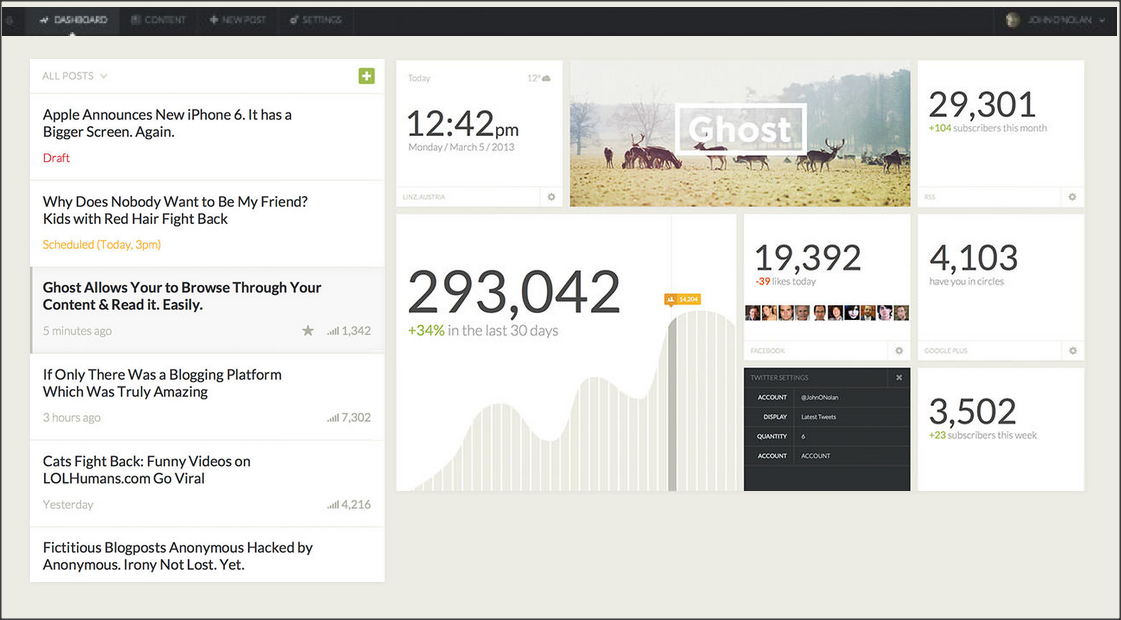
\includegraphics[width=\textwidth]{ghost_dash}
\caption{Ghost Dashboard}
\end {figure}